\documentclass[usenames,dvipsnames,tikz]{standalone}
\usepackage{amsmath,amssymb}
\usepackage{xcolor}
\colorlet{tBlue}{RoyalBlue!35!Cerulean}
\colorlet{tRed}{Red}
\usepackage{tikz}
\usepackage{standalone}
\begin{document}
	
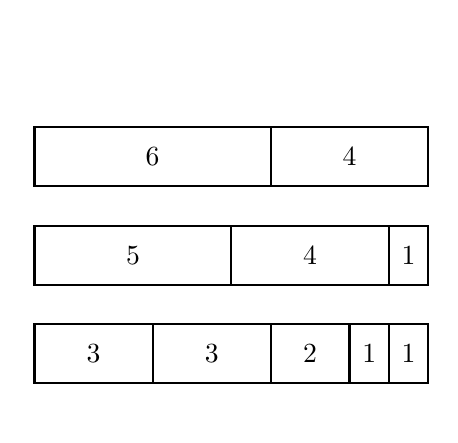
\begin{tikzpicture}
%\draw [help lines] (-1,-2) grid (13,5);
% 1=0.1, 2=0.15, 3=0.2, 4=0.25, 5=0.3
% 6, 5, 4, 4, 3, 3, 2, 1, 1, 1.

% BPP
\draw [thick] (0,0) rectangle (5,0.75);
\draw [thick] (0,1.25) rectangle (5,2);
\draw [thick] (0,2.5) rectangle (5,3.25);
\draw [thick, white] (0,3.75) rectangle (5,4.5);
 
% Bottom row, 3, 3, 2, 1
\draw [thick] (1.5,0) -- (1.5,0.75);
\draw [thick] (3,0) -- (3,0.75);
\draw [thick] (4,0) -- (4,0.75);
\draw [thick] (4.5,0) -- (4.5,0.75);
\node at (0.75, 0.375) {3};
\node at (2.25, 0.375) {3};
\node at (3.5, 0.375) {2};
\node at (4.25, 0.375) {1};
\node at (4.75, 0.375) {1};

% Middle row, 5, 4, 1
\draw [thick] (2.5,1.25) -- (2.5,2);
\draw [thick] (4.5,1.25) -- (4.5,2);
\node at (1.25, 1.625) {5};
\node at (3.5, 1.625) {4};
\node at (4.75, 1.625) {1};

% Top row, 6, 4
\draw [thick] (3,2.5) -- (3,3.25);
\node at (1.5, 2.875) {6};
\node at (4, 2.875) {4};

\node [below] at (0.1,0) {\textcolor{white}{\scriptsize{1}}};
\node [below] at (1.25,0) {\textcolor{white}{\scriptsize{4}}};
\node [below] at (1.65,0) {\textcolor{white}{\scriptsize{3}}};
\node [below] at (1.9,0) {\textcolor{white}{\scriptsize{1}}};

\end{tikzpicture}

\end{document}